\documentclass[class=report, float=false, crop=false]{standalone}
\usepackage[subpreambles=true]{standalone}

\usepackage{pgf, tikz}
\usetikzlibrary{shapes.misc}
\usetikzlibrary{decorations.pathreplacing}

\tikzset{cross/.style={cross out, draw=black, minimum size=2*(#1-\pgflinewidth), inner sep=0pt, outer sep=0pt},
%default radius will be 1pt. 
cross/.default={0.25pt},
    point/.style={
    thick,
    draw=black,
    cross out,
    inner sep=0pt,
    minimum width=4pt,
    minimum height=4pt,
    },
}

\graphicspath{{figures/images/}}

% \begin{cbunit}

\begin{document}

\chapter{Jamming}
\label{chap:jamming}

Many recent works have studied the properties of the jamming transition for packings of 2D and 3D soft- and hard-core spherical particles. Our goal here is to investigate how these properties are affected when considering spheroids.\\

We will first introduce the jamming transition and the models and methods that have been involved to study this transition for spheres and then present the modifications we have brought to these in order to study rotating spheroids, based on the theoretical knowledge and numerical methods we have summarised on \hyperref[chap:quaternions]{quaternions} and \hyperref[chap:ellipsoids]{ellipsoids}.

\section{Jamming transition}

\subsection{Phenomenon}
\label{jamming_phenomenon}

A few decades ago, little was still known about granular materials. According to Pierre-Gilles de Gennes, "granular matter in 1998 [was] at the level of solid state physics in 1930." \cite{de1999granular} Yet, these materials are of great theoretical interest in the domain of statistical physics \cite{kadanoff1999built}.\\

What has been observed is that granular materials develop a yield stress in a disordered state \cite{PRE68.011306} -- or a stress relaxation time which exceeds a reasonable experimental time -- upon increasing the packing fraction $\phi$ above a critical value $\phi_J$. At low $\phi$, each particle can move independently of its neighbours while at high $\phi$ the particles can not avoid each other, resulting in a bulk modulus since the pressure increases upon compression. This phenomenon is called jamming and corresponds to a transition from a flowing liquid-like state to an amorphous rigid solid state.\\

Jamming is encountered everywhere, whether it is unintended -- \textit{e.g.}, grains and beans jam in hoppers \cite{youtube1,youtube2,to2001jamming}, cars jam on the highway \cite{eisenblatter1998jamming} -- or purposefully put into practice in engineering applications -- \textit{e.g.}, to easily, efficiently and reliably hold objects \cite{youtube3,brown2010universal}.\\

The phenomenon is also present in other systems with other control parameters \cite{d2001jamming}. Foams jam upon decreasing the applied shear stress and supercooled liquids jam upon decreasing the temperature -- the latter phenomenon being already known as the glass transition from a flowing liquid to a frozen glass.\\

These observations led Liu and Nagel to hypothesise that they are controlled by the same mechanisms \cite{liu1998nonlinear}, and thus to summarise them in a phase diagram \cite{PRE68.011306} which axis are the aforementioned parameters: temperature $T$, shear stress $\sigma$ and packing fraction $\phi$ (figure \ref{phase_diagram_jamming}). The surface below which states are jammed corresponds to the points for which the system behaves like a solid on any experimental time scale and the point J is meant to correspond to the packing fraction $\phi_J$ at which the system at $T=0$ and $\sigma=0$ jam in the thermodynamic limit (infinite system, \textit{i.e.}, $N\rightarrow+\infty$).

\begin{figure}[h!]
\centering
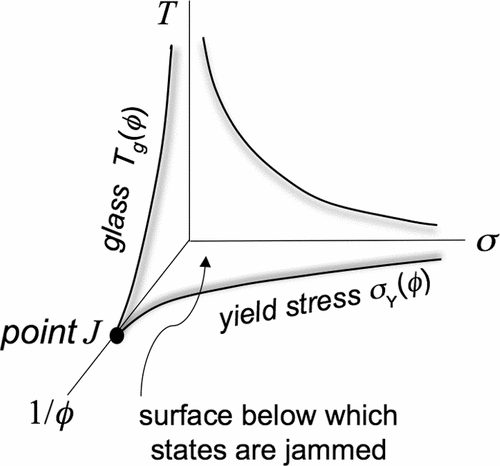
\includegraphics[width=0.28\textwidth]{figures/images/phase_diagram.png}
\caption{\textit{source:} \cite{PRE83.031307}}
\label{phase_diagram_jamming}
\end{figure}

Defining what is exactly a "jammed system" is a problem of great mathematical and physical interest \cite{torquato2001multiplicity,donev2004unusually}, in particular it has finally allowed physicists to replace the concept of random close packing (RCP) with the more rigorous and precise concept of maximally random jammed (MRJ) state \cite{torquato2000random}. We will however set aside these considerations to rather focus on the critical behaviours (parts \ref{critical_behaviour}, \ref{relaxation_time} and \ref{contact_number}) observed at the transition to such a state.

\subsection{Critical behaviour}
\label{critical_behaviour}

In the vicinity of $J$, we have that the shear viscosity $\eta \equiv \sigma/\dot{\gamma}$ -- with $\sigma$ the shear stress and $\dot{\gamma}$ the shear strain rate, -- or equivalently the pressure viscosity $\eta_p \equiv p/\dot{\gamma}$ -- with $p$ the pressure, -- and a correlation length scale $\xi$ diverge as
\begin{equation}
\boxed{
\begin{aligned}
\eta,\eta_p \isEquivTo{\phi\rightarrow\phi_J} \left|\phi - \phi_J\right|^{-\beta}\\
\xi \isEquivTo{\phi\rightarrow\phi_J} \left|\phi - \phi_J\right|^{-\nu}
\end{aligned}
}
\label{critical_exponents}
\end{equation}
for $\phi \lessgtr \phi_J$ for soft-core particles in the limit $\dot{\gamma}\rightarrow0$ \cite{PRL99.178001,PRE83.030302} and for $\phi < \phi_J$ for hard-core particles \cite{PRL109.108001}. We will always assume that these exponents have the same value for whatever sign of $\phi-\phi_J$.\\

Using $\eta_p$ rather than $\eta$ has been proven to reduce errors due to necessary corrections to scaling \cite{PRE83.030302}. Moreover, we have to keep in mind that equation \ref{critical_exponents} holds only very close to $\phi_J$. Since the dimensionless friction $\mu \equiv \eta/\eta_p$ has a strong $\phi$-dependence, corrections may have to be added to the scaling for larger packing fractions intervals \cite{PRE83.030302,PRE91.062209}. Please refer to part \ref{scaling_analysis} for more details on the scaling methods.\\

This power-law divergence of the transport coefficient and of a correlation length scale are reminiscent of the behaviour near a critical point \cite{PRE83.030302,plischke1994equilibrium,PRE83.030303} of a second-order continuous phase transition.\\

The original conjecture of the authors of \cite{PRE68.011306} was that $J$ was indeed a critical point which "may control the region around it and thereby govern the nature of the entire jamming surface in the phase diagram." This point would then be the athermal jamming point corresponding to the $T\rightarrow0$ limit of the equilibrium glass transition curve in the $(1/\phi,T)$ plane. However, it was later suggested that the equilibrium glass transition would be governed by a critical point distinct from $J$ \cite{PRE83.031307}.

\subsection{Finite-size effects}

For a finite number $N$ of particles, the system will jam at a packing fraction $\phi$ somewhat below $\phi_J$ because there is always a finite probability to find a configuration with a force chain spanning the width of the system, causing the system to jam.\\

When shearing a packing of particles the system explores an increasing region of configuration space, it will thus eventually find a configuration causing it to jam. The statistical weight of these configurations, associated with the time required for the system to jam, decreases as one decreases the packing fraction $\phi$ or increases the number of particle $N$. Therefore, in the limit of a infinite system $N\rightarrow+\infty$, it is expected that the system jam in a finite time only for $\phi\geq\phi_J$ \cite{PRL99.178001}.

\subsection{Relaxation time}
\label{relaxation_time}

For a packing of soft-core particles at a density $\phi<\phi_J$ in the thermodynamic limit $N\rightarrow+\infty$, the state of minimum energy will always be a state where the particles do not overlap, therefore a state of zero energy and zero pressure. When one applies a constant shear strain rate to such a system, the particles overlap and the energy becomes non-zero. One can then be interested in the decay of the energy and the pressure when the shearing ceases.\\

Authors of \cite{PRE91.062209} studied this decay for systems of soft-core disks with harmonic elastic interactions (see part \ref{model_soft_core}) at constant shear strain rate. What they have observed is that after a short transient time, the pressure decays exponentially to zero with a characteristic time scale $\tau(\phi,\dot{\gamma})$
\begin{equation}
\boxed{
p(t) \sim \exp\left(-t/\tau(\phi,\dot{\gamma})\right)
}
\end{equation}
which they called the \textit{relaxation time}. This relaxation time increases with increasing initial shear strain rate $\dot{gamma}$ for a given $\phi$ and diverges as $\phi$ approaches $\phi_J$ from below.\\

Another relevant time scale presented by the authors is the \textit{dissipation time} $\tau_{\text{diss}}(\phi,\dot{\gamma})$, which represents the initial decay rate of the energy. It is obtained by taking the ratio of the energy $E$ by the dissipated power $P_{\text{diss}}$. If the system is steadily sheared, then $P_{\text{diss}}$ equals the input power $P_{\text{in}} \sim \sigma\dot{\gamma}$ with $\sigma$ the shear stress. Therefore, $\tau_{\text{diss}}(\phi,\dot{\gamma}) \sim E/\sigma\dot{\gamma}$.\\

Since that, for harmonic elastic interactions, we have $p\sim\delta$ and $E\sim\delta^2$ with $\delta$ the overlap, we then expect the energy to decay exponentially with a characteristic time scale $\tau(\phi,\dot{\gamma})/2$. In consequence, the authors chose
\begin{equation}
\boxed{
\tau_{\text{diss}}(\phi,\dot{\gamma}) = 2\frac{E}{\sigma\dot{\gamma}}
}
\end{equation}
for this time scale to be compared with $\tau(\phi,\dot{\gamma})$. Contrarily to the relaxation time, the dissipation time decreases with increasing initial shear strain rate $\dot{\gamma}$, but also diverges as $\phi$ approaches $\phi_J$ from below.\\

Indeed, if we notice that
\begin{align*}
\tau_{\text{diss}} = 2\frac{E}{\sigma\dot{\gamma}} \sim \frac{E/\dot{\gamma}^2}{\sigma/\dot{\gamma}} \sim \frac{(p/\dot{\gamma})^2}{\sigma/\dot{\gamma}} \sim \frac{\eta_p^2}{\eta} 
\end{align*}
we can directly infer from equation \ref{critical_exponents} that
\begin{equation}
\boxed{
\tau_{\text{diss}} \isEquivTo{\phi\rightarrow\phi_J} (\phi_J-\phi)^{—\beta}
}
\label{tdiss}
\end{equation}
therefore, the dissipation time diverges with the same exponent as the viscosity and its pressure equivalent.\\

Authors of \cite{PRE91.062209} finally showed that in the limit of low initial shear strain rate $\dot{\gamma}\rightarrow0$, the relaxation time and the dissipation time behave essentially the same close to $\phi_J$
\begin{equation}
\tau \isEquivTo{\subalign{\dot{\gamma}&\rightarrow0 \\ \phi&\rightarrow\phi_J}} \tau_{\text{diss}}
\label{ttdiss}
\end{equation}
therefore the relaxation time also diverges with the critical exponent $\beta$.\\

We emphasise that equations \ref{tdiss} and \ref{ttdiss} give, in addition to the study of the quantities in equation \ref{critical_exponents}, a way to determine the critical exponent associated with the divergence of the viscosity at the jamming transition.\\

It was then suggested that $\tau$ may be a fundamental quantity which controls the overlap $\delta/\dot{\gamma}$ and thus would be behind the divergence of the transport coefficients.

\subsection{Contact number}
\label{contact_number}

Many works have focused on determining the coordination number $z$ -- \textit{i.e.}, the number of contacts per particle -- for static packings near the jamming transition.\\

An important result is that disordered packings of disks and spheres are isostatic at jamming \cite{PRE68.011306,PRL88.075507,PRE91.062209}, meaning that the total number of contacts is equal to the total number of degrees of freedom \cite{alexander1998amorphous}, then leading to a completely statically defined system -- however, one has to remove rattlers, \textit{i.e.} particles with less than 3 contacts which are then not locked up at a fixed position, from the calculation. With $d_f$ the number of degrees of freedom, we then have the isostatic contact number, $z_{\text{iso}}=2d_f$, where $d_f$  equals to 2 for disks and 3 for spheres (translational degrees of freedom).\\

Moreover, the difference of the contact number to its isostatic value $\delta z \equiv z_{\text{iso}} - z$ vanishes algebrically when the packing fraction approaches its jamming value $\phi_J$ from below
\begin{equation}
\delta z \isEquivTo{\phi\rightarrow\phi_J} (\phi_J - \phi)^{u_z}
\label{deltaz_vanish}
\end{equation}
which with equations \ref{tdiss} and \ref{ttdiss} leads to
\begin{equation}
\tau \isEquivTo{\subalign{\dot{\gamma}&\rightarrow0 \\ \phi&\rightarrow\phi_J}} \delta z^{-\beta/u_z}
\label{tau_dz_scaling}
\end{equation}
for soft-core particles near the hard-core limit, according to \cite{PRE91.062209}.\\

Authors of \cite{PRE91.062209}, whose method is described in part \ref{method_relaxation}, emphasised the following results from their study of the relaxation of sheared packings of soft-core frictionless disks:
\begin{itemize}
\item the contact number always decreases in the relaxation process,
\item this change is bigger when increasing the initial shear rate,
\item the contact number after relaxation decreases slowly with decreasing initial shear rate,
\item the contact number in sheared packings can be above isostaticity while the contact number after relaxation is always below.\\
\end{itemize}

It has been suggested that packings of non-spherical particles do not satisfy this isostaticity property \cite{donev2007underconstrained} and in particular that jammed packings of frictionless ellipsoids are hypostatic \cite{donev2004improving}, \textit{i.e.} exhibit a contact number at jamming lesser than its isostatic value.\\

The contact number and especially its critical value at jamming, alongside with the jamming packing fraction, are thought to be at the origin of the critical behaviours of the mechanical properties of frictionless packings of spherical and ellipsoidal particles \cite{van2009jamming}.

\subsection{Orientational ordering}

Considering non-spherical particles breaks down the isotropy of the rotation phase space. Therefore one can expect that, near the jamming transition, a system of ellipsoidal particles would develop a significant orientational ordering.\\

Nonetheless, it has been suggested that packings of ellipsoidal particles showed no such ordering at jamming in static simulations \cite{donev2004improving} but one can still hypothesise that such a phenomenon is to be expected in shearing simulations.

\subsection{Universality}

A frequent question in statistical physics is whether different critical phenomena -- observed in identical or different systems -- behave similarly, which is characterised by them having the same critical exponents. Such similar phenomena are said to belong to an unique \textit{universality class}. It was empirically found that the elements of an universality class were linked by their spatial dimensionality and the symmetry of their ordered phase \cite{plischke1994equilibrium}.\\

It was showed that different models for the dissipation of the energy in packings of soft-core spheres did not influence the critical exponents characterising the jamming transition \cite{PRL113.148002,PRE91.062209}, while different models for the elastic interaction between particles did \cite{PRE68.011306}. Moreover, it was suggested that the critical exponent characterising the vanishing of the excess contact number to isostaticity was independent of both the spatial dimensionnality of the packing and the elastic interaction considered for soft-core spheres \cite{PRE68.011306}.\\

When considering ellipsoidal particles, it would be interesting to determine how the asphericity of the particles influences the critical exponents of the jamming transition and whether systems of oblate and prolate spheroids behave the same.

\section{Methods}

\subsection{Jamming transition}
\label{methods_jamming_transition}

Many numerical methods have been used to study the jamming of a system of spherical particles:
\begin{itemize}
\item Most of them consist of evaluating and studying the proportion of jammed states as a function of the density and infer from these data the jamming packing fraction. What distinguishes the methods is then the way the system is prepared:
\begin{itemize}
\item Relaxation from initially random states simulations \cite{PRE83.031307,PRE83.030303}. A system corresponding to a completely random state ($T=+\infty$) is cooled by using energy minimisation techniques.
\item Quasistatic shearing \cite{PRE83.030303}. A system of which the energy has been initially minimised is gradually sheared, with energy minimisation steps between each increment of the shear strain.
\item Compression \cite{PRL104.165701}.
\end{itemize}
\item Other methods are based on the shearing at constant shear rate of a given system \cite{PRL99.178001}, which can be performed using Lees-Edwards periodic boundary conditions \cite{lees1972computer,morriss2013statistical}. From the assumption of a critical behaviour of the mechanical properties (\textit{e.g.}, pressure, shear modulus) near the jamming point $J$, the scaling analysis of the behaviour of the system enables one to infer the jamming packing fraction and the critical exponents.
\end{itemize}
However, there appears to have little agreement in the values for the jamming density and of the critical exponents found in the literature. This is thought to be caused by the neglect of corrections to scaling in these papers \cite{PRE83.030302}. Moreover, in relaxation and compression protocols, particles tend to order themselves into clusters. This leads to values of the jamming density which are dependent of the way the samples were prepared and treated -- a dependence which is often to be expected when studying granular materials \cite{vanel1999memories,toiya2004transient}. Some authors suggested that, since $\phi_J$ was history-dependent, the point J may be ill-defined, even when clustering plays no role \cite{PRL104.165701}.\\

We can note that, to avoid crystallisation, most simulations involve polydispersity \cite{PRL104.165701}.\\

On the contrary, the process of shearing -- no matter how slow -- breaks the clustering at the origin of varying and higher than expected values of $\phi_J$. It has then been showed that quasistatic shearing protocols lead to an unique -- well-defined -- value of the jamming density $\phi_J$, corresponding to the jamming density for shearing simulations in the limit of vanishing shear strain rate, which does not depend on the initial configuration or the details of the shearing protocol \cite{PRE83.031307}.\\

It has then been proposed to study jamming in the $(1/\phi,T,\dot{\gamma})$ phase space -- where $\dot{\gamma}$ is the shear strain rate -- where $J$ would be unique. In such a phase space, the $(1/\phi,T)$ plane at $\dot{\gamma} \rightarrow 0$ corresponds to the plane of quasistatically sheared steady states.

\subsection{Relaxation time}
\label{method_relaxation}

To study the relaxation time $\tau(\phi,\dot{\gamma})$ of a system of soft-core particles, the authors of \cite{PRE91.062209} made use of a 2-stage process. First, the system is driven at steady shear with the constant shear strain rate $\dot{\gamma}$. Then, the shearing is stopped but the dynamics is continued until the system relaxes down to a minimum energy.

\subsection{Soft- to hard-core mapping}
\label{softtohard}

Shearing simulations are more or less easily conducted with soft-core particles. We can be interested to know how the data from these simulation can be used to study the rheological behaviour of packings of hard-core particles near the jamming transition.\\

We can find in \cite{PRL109.108001} a method to map soft-core particles at a given packing fraction $\phi$ and shear strain rate $\dot{\gamma}$ to equivalent hard-core particles at a lesser packing fraction $\phi_{\text{eff}}$ such as
\begin{equation}
\begin{aligned}
\eta^s_p(\phi,\dot{\gamma}) &= \eta^s_p(\phi_{\text{eff}},\dot{\gamma}\rightarrow0)\\
\eta^h_p(\phi_{\text{eff}}) &\equiv \eta^s_p(\phi_{\text{eff}},\dot{\gamma}\rightarrow0) \isEquivTo{\phi_{\text{eff}}\rightarrow\phi_J} \left(\phi_J - \phi_{\text{eff}}\right)^{-\beta}
\label{phieff}
\end{aligned}
\end{equation}
according to equation \ref{critical_exponents}. We denoted $\eta_s$ and $\eta_p$ are the pressure equivalents of viscosity for packings of soft- and hard-core particles respectively.\\

This mapping is done by assuming that $\phi_{\text{eff}}$ is determined by the extent of particle overlaps, measured by the average energy per particle $E(\phi,\dot{\gamma})$. Authors of \cite{PRL109.108001} then proposed the following relation
\begin{equation}
\phi_{\text{eff}}(\phi,\dot{\gamma}) = \phi - h(E(\phi,\dot{\gamma}))
\label{phieff_}
\end{equation}
where $h$ can be determined asymptotically close to $\phi_J$.\\

We can first notice that there is no distinction between soft-core and hard-core particles in a system where the particles do not overlap. In such a system, the average energy per particle equals to $0$, therefore we must have
\begin{equation}
h(0)=0
\end{equation}

In a jammed system -- \textit{i.e.}, $\phi\ge\phi_J$ -- of soft-core particles, particles have no choice but to overlap leading to $p > 0$ even as $\dot{\gamma} \rightarrow 0$, and then $\eta_p^s(\phi\ge\phi_J,\dot{\gamma}\rightarrow0)\rightarrow+\infty$. In consequence, according to equation \ref{phieff}, we must have $\eta^h_p(\phi_{\text{eff}})\rightarrow+\infty$, which is only achieved for a system of hard-core particles at $\phi_{\text{eff}}=\phi_J$, therefore
\begin{equation}
\begin{aligned}
\phi_{\text{eff}}(\phi\ge\phi_J,\dot{\gamma}\rightarrow0) = \phi_J\\
\end{aligned}
\label{phiefflimit}
\end{equation}

From equations \ref{phieff_} and \ref{phiefflimit}, we have that
\begin{align*}
\phi_{\text{eff}}(\phi\ge\phi_J,\dot{\gamma}\rightarrow0) = \phi - h(E(\phi,\dot{\gamma}\rightarrow0)) = \phi_J \Rightarrow h(E(\phi,\dot{\gamma}\rightarrow0)) = \phi-\phi_J
\end{align*}
and, since $E(\phi,\dot{\gamma}\rightarrow0)$ vanishes algebraically close to $\phi_J$, we can write
\begin{align*}
E(\phi,\dot{\gamma}\rightarrow0) \isEquivTo{\phi\rightarrow\phi_J} (\phi-\phi_J)^{y_E} &\Leftrightarrow E(\phi,\dot{\gamma}\rightarrow0)^{1/y_E} \isEquivTo{\phi\rightarrow\phi_J} \phi-\phi_J\\
&\Rightarrow E(\phi,\dot{\gamma}\rightarrow0)^{1/y_E} \isEquivTo{\phi\rightarrow\phi_J} h(E(\phi,\dot{\gamma}\rightarrow0))\\
&\Rightarrow X^{1/y_E} \isEquivTo{X\rightarrow0} h(X)
\end{align*}
where the latter equivalence can be applied to $E(\phi,\dot{\gamma})$ in the vicinity of $\phi_J$, therefore
\begin{equation}
\boxed{
\phi_{\text{eff}}(\phi,\dot{\gamma})\operatorname*{~=~}_{\phi\rightarrow\phi_J}\phi-cE(\phi,\dot{\gamma})^{1/y_E}
}
\label{phieff_soft2hard}
\end{equation}
with $c$ a constant.

\section{Model of frictionless soft-core particles}
\label{model_soft_core}

\subsection{Interactions between spherical particles}

Much work on jamming has focused on a model of athermal, frictionless and spherical soft-core particles with repulsive contact interaction proposed by D. J. Durian to describe foam mechanics \cite{durian1995foam}, in which the rotational motion of the particles does not play any role. For two spheres $\mathcal{S}_i$ and $\mathcal{S}_j$, this model gives the following elastic potential of interaction
\begin{equation}
\boxed{
\mathcal{V}_{ij}(r_{ij}) = \begin{cases} \frac{1}{2} k_e (1 - r_{ij}/d_{ij})^2 &\text{ if } r_{ij} \leq d_{ij} \Leftrightarrow \mathcal{S}_i \cap \mathcal{S}_j \neq \emptyset \\ 0 &\text{ if } r_{ij} > d_{ij} \Leftrightarrow \mathcal{S}_i \cap \mathcal{S}_j = \emptyset \end{cases}
}
\label{elastic_spheres}
\end{equation}
where $\vec{r_{i/j}}$ and $R_{i/j}$ are the positions and the radii of $\mathcal{S}_i$ and $\mathcal{S}_j$, $r_{ij} = ||\vec{r_i} - \vec{r_j}||$ and $d_{ij} = R_i + R_j$.\\

This potential of interaction thus leads to the following force exterted on $\mathcal{S}_i$ by $\mathcal{S}_j$
\begin{equation}
\boxed{
\vec{f}_i^{\text{el}}(r_{ij}) = \begin{cases} {\textstyle - \frac{k_e}{d_{ij}}} (1 - r_{ij}/d_{ij})~\hat{r_{ij}} &\text{ if } \mathcal{S}_i \cap \mathcal{S}_j \neq \emptyset \\ 0 &\text{ if } \mathcal{S}_i \cap \mathcal{S}_j = \emptyset
\end{cases}
}
\label{elastic_force_spheres}
\end{equation}
where $\hat{r_{ij}} = (\vec{r_i} - \vec{r_j})/||\vec{r_i} - \vec{r_j}||$.\\

The original idea of Durian was to model the interaction between two bubbles in contact by the compression of two springs in series which constants would scale with the Laplace pressures, $\textit{i.e.}$ inversely proportionnal to the bubbles' radii, hence the harmonic potential.\\

Because of the finite range of the interactions, the potential energies vanish at a fixed finite radius, therefore this system is a good starting point to study macroscopic granular or colloidal systems, suspensions, foams, emulsions and liquids \cite{PRE68.011306,PRL113.148002}.\\

When simulating the shearing dynamics of such a system, one has to introduce a way to dissipate the energy. This can be done with either one of these 2 manners, also proposed by Durian \cite{durian1995foam,PRL113.148002} :
\begin{itemize}
\item A contact dissipation (CD) which is a pairwise interaction, additive and proportional to the difference of the velocities of the moving particles in contact,
\begin{equation}
\boxed{
\vec{f}_{\text{CD},i}^{\text{dis}} = -k_d \sum_{\mathclap{j\text{ neighbours}}} \left(\vec{v_i} - \vec{v_j}\right)
}
\label{fdis_cd}
\end{equation}
where $\vec{v_i}$ denotes the velocity of the particle $i$. This was originally meant to model the dissipation in the liquid between moving bubbles.
\item A reservoir dissipation (RD), which is a mean-field approximation of CD where the pairwise difference of the velocities is replaced for each particle by a dissipation with respect to the average shear flow of the background reservoir,
\begin{equation}
\boxed{
\vec{f}_{\text{RD},i}^{\text{dis}} = -k_d \left(\vec{v_i} - \dot{\gamma}y_i\vec{e_x}\right)
}
\label{fdis_rd}
\end{equation}
where $\vec{v_i}$ and $y_i$ denote the velocity and ordinate of the particle $i$, and $\dot{\gamma}$ and $\vec{e_x}$ denote the shearing strain rate and direction.
\end{itemize}
Therefore the translational motion of the particles is described by
\begin{equation}
m_i \dot{\vec{v_i}} = \vec{f}_i^{\text{el}} + \vec{f}_i^{\text{dis}}
\end{equation}
To neglect the effects of inertia, we have to consider the overdamped limit $m_i \rightarrow 0$, which is easily done in the RD model. For the CD model, it is numerically necessary to take a finite value of the mass, therefore the overdamped limit has to be verified \textit{a posteriori} \cite{PRL113.148002}.

\subsection{Elastic force between ellipsoids}
\label{elastic_force_part}

\subsubsection{Reformulation of the elastic potential of interaction for spheres}
\label{reformulation_elastic}

The distance between the centres of two ellipsoids is not directly relevant to the intensity of their interactions. We need to reformulate equation \ref{elastic_spheres} with parameters which would be relevant for ellipsoids. In \cite{donev2007underconstrained}, the overlap potential of two ellipsoids is a function of $\mu$ the rescaling factor by which the particles need to be resized in order to be externally tangent. We can investigate whether the equation \ref{elastic_spheres} can be reformulate as a function of such a number.\\

First of all, we can show that if two spheres $\mathcal{A}$ and $\mathcal{B}$, of centres $A \equiv \vec{r_A}$ and $B \equiv \vec{r_B}$ and of radii $R_A$ and $R_B$ respectively, are externally tangent and that none of these spheres is entirely contained in the other, then their point of contact is located on the $[AB]$ line segment. Indeed, if we denote $C$ their point of contact and assume it is not on the $[AB]$ line segment, then
\begin{align*}
||AB|| < ||AC|| + ||BC||
\end{align*}
If we denote $U$ and $V$ the intersection of the $[AB]$ line segment with $\mathcal{A}$ and $\mathcal{B}$ respectively, then
\begin{align*}
||AB||&= ||AU|| + ||UV|| + ||VB|| < ||AC|| + ||BC||
\end{align*}
Since $U,C \in \mathcal{A}$ and $V,C \in \mathcal{B}$, then
\begin{align*}
||AU|| = ||AC|| \text{ and } ||VB|| = ||BC|| \Rightarrow ||UV|| < 0
\end{align*}
which is not possible, therefore their point of contact $C$ have to be on the $[AB]$ line segment.\\

We we will denote $\forall \vec{r} \in [AB]$, $\mu_A(\vec{r})$ and $\mu_B(\vec{r})$ the rescaling factor that has to be applied to $\mathcal{A}$ and $\mathcal{B}$ respectively for $\vec{r}$ to be on their surface. Then
\begin{align*}
1 &= \frac{||\vec{r} - \vec{r_A}||}{\mu_A(\vec{r})R_A} \Leftrightarrow \mu_A(\vec{r}) = \frac{||\vec{r} - \vec{r_A}||}{R_A}\\
1 &= \frac{||\vec{r} - \vec{r_B}||}{\mu_B(\vec{r})R_B} \Leftrightarrow \mu_B(\vec{r}) = \frac{||\vec{r} - \vec{r_B}||}{R_B}
\end{align*}
Moreover, since $\vec{r} \in [AB]$ we have
\begin{equation}
\begin{aligned}
&\vec{r} = \vec{r_A} + \mu_A(\vec{r})R_A \frac{\vec{r_B}-\vec{r_A}}{||\vec{r_B}-\vec{r_A}||}\\
&\vec{r} = \vec{r_B} + \mu_B(\vec{r})R_B \frac{\vec{r_A}-\vec{r_B}}{||\vec{r_A}-\vec{r_B}||}
\label{scale_spheres}
\end{aligned}
\end{equation}
We are now looking for the point $\vec{r_C} \in [AB]$ which satisfies $\mu_A(\vec{r}_C) = \mu_B(\vec{r}_C) = \mu(\vec{r_{\mathcal{A}}},\vec{r_{\mathcal{B}}})$. For such a point we have
\begin{equation}
\begin{aligned}
\vec{r_C} = \vec{r_C} \Leftrightarrow& \vec{r_A} + \underbrace{\mu_A(\vec{r_C})}_{\mu(\vec{r_{\mathcal{A}}},\vec{r_{\mathcal{B}}})}R_A \frac{\vec{r_B}-\vec{r_A}}{||\vec{r_B}-\vec{r_A}||} = \vec{r_B} + \underbrace{\mu_B(\vec{r_C})}_{\mu(\vec{r_{\mathcal{A}}},\vec{r_{\mathcal{B}}})}R_B \frac{\vec{r_A}-\vec{r_B}}{||\vec{r_A}-\vec{r_B}||}\\
\Leftrightarrow& (\vec{r_A} - \vec{r_B})||\vec{r_A} - \vec{r_B}|| = \mu(\vec{r_{\mathcal{A}}},\vec{r_{\mathcal{B}}})(\vec{r_A} - \vec{r_B})(R_A + R_B)\\
\xRightarrow[\vec{r_A}\neq\vec{r_B}]{}& \mu(\vec{r_{\mathcal{A}}},\vec{r_{\mathcal{B}}}) = \frac{||\vec{r_A}-\vec{r_B}||}{R_A + R_B}
\label{rc_spheres}
\end{aligned}
\end{equation}
What we have just showed is that for two spheres $\mathcal{S}_i$ and $\mathcal{S}_j$ there exists a point $\vec{r_C}$ on the segment connecting their centres for which $\mu_i(\vec{r_C}) = \mu_j(\vec{r_C}) = \mu(\vec{r_C}) = r_{ij}/d_{ij}$. Therefore, we can reformulate equation \ref{elastic_spheres}
\begin{equation}
\boxed{\mathcal{V}_{ij}(\vec{r_i},\vec{r_j}) = \begin{cases} \frac{1}{2} k_e (1 - \mu(\vec{r_i},\vec{r_j}))^2 &\text{ if } \mathcal{S}_i \cap \mathcal{S}_j \neq \emptyset\\ 0 &\text{ if } \mathcal{S}_i \cap \mathcal{S}_j = \emptyset \end{cases}}
\label{elastic_potential}
\end{equation}
We can verify that this new formulation leads to the same elastic force that in equation \ref{elastic_force_spheres}. If we denote $\vec{f}_{ij}^{\text{el}}$ the elastic force exerted on $\mathcal{S}_i$ by $\mathcal{S}_j$, then we should have
\begin{align*}
\vec{f}_{ij}^{\text{el}} = -\frac{d\mathcal{V}_{ij}}{d\vec{r_i}}(\vec{r_i},\vec{r_j}) = k_e(1 - \mu(\vec{r_i},\vec{r_j}))\frac{d\mu}{d\vec{r_i}}(\vec{r_i},\vec{r_j})
\end{align*}
From equation \ref{scale_spheres} we can infer
\begin{align*}
\frac{d\mu_i}{d\vec{r_i}}(\vec{r_i},\vec{r_j}) = -\frac{1}{R_i}\frac{\vec{r_j} - \vec{r_i}}{||\vec{r_j} - \vec{r_i}||}
\end{align*}
and from equation \ref{rc_spheres}
\begin{align*}
\vec{r_C} &= \vec{r_i} + \mu R_i \frac{\vec{r_j} - \vec{r_i}}{||\vec{r_j} - \vec{r_i}||}\\
&=  \vec{r_i} + \frac{\cancel{||\vec{r_j} - \vec{r_i}||}}{R_i + R_j} R_i \frac{\vec{r_j} - \vec{r_i}}{\cancel{||\vec{r_j} - \vec{r_i}||}}\\
&= \vec{r_i} + R_i \frac{\vec{r_j} - \vec{r_i}}{R_i + R_j} 
\end{align*}
therefore $\frac{d\mu}{d\vec{r_i}}(\vec{r_C}) = \frac{1}{R_i + R_j}\frac{\vec{r_i} - \vec{r_j}}{||\vec{r_i} - \vec{r_j}||} = \frac{1}{d_{ij}}\frac{\vec{r_i} - \vec{r_j}}{||\vec{r_i} - \vec{r_j}||}$. Finally, we have the correct expression for the elastic force
\begin{equation}
\vec{f}_{ij}^{\text{el}} = \frac{k_e}{d_{ij}}\left(1 - \frac{r_{ij}}{d_{ij}}\right)\frac{\vec{r_i} - \vec{r_j}}{||\vec{r_i} - \vec{r_j}||}
\label{forces_spheres_olsson}
\end{equation}
corresponding to equation \ref{elastic_force_spheres}.

\subsubsection{Elastic force between ellipsoids}

We will assume that the equation \ref{elastic_potential} remains valid for two ellipsoids $\mathcal{A}$ and $\mathcal{B}$.

\begin{equation}
\boxed{\mathcal{V}_{\mathcal{A}\mathcal{B}}(\vec{r_{\mathcal{A}}},\vec{r_{\mathcal{B}}}) = \begin{cases} \frac{1}{2} k_e (1 - \mu(\vec{r_{\mathcal{A}}},\vec{r_{\mathcal{B}}}))^2 &\text{ if } \mathcal{A} \cap \mathcal{B} \neq \emptyset\\ 0 &\text{ if } \mathcal{A} \cap \mathcal{B} = \emptyset \end{cases}}
\label{elastic_potential_ellipsoid}
\end{equation}

Let $\bar{B}_{\mathcal{A}}$ be the reduced belonging matrix of $\mathcal{A}$, $\vec{r_{\mathcal{A}}}$ its centre and $\vec{r_C}$ the point of external tangency of ellipsoids $\mathcal{A}$ and $\mathcal{B}$ when rescaled by a common rescaling factor $\mu(\vec{r_{\mathcal{A}}},\vec{r_{\mathcal{B}}})$, then
\begin{equation}
\mu^2(\vec{r_{\mathcal{A}}},\vec{r_{\mathcal{B}}}) = (\vec{r_C} - \vec{r_{\mathcal{A}}})^T\bar{B}_{\mathcal{A}}(\vec{r_C} - \vec{r_{\mathcal{A}}})
\label{mu2_ellipsoids}
\end{equation}
according to equation \ref{belonging_function_reduced}.\\

According to equation \ref{elastic_potential_ellipsoid}, the force exerted on $\mathcal{A}$ by $\mathcal{B}$ is
\begin{equation}
\begin{aligned}
\vec{f}_{\mathcal{A}\mathcal{B}}^{\text{el}}(\vec{r_{\mathcal{A}}},\vec{r_{\mathcal{B}}}) &= - \frac{d\mathcal{V}_{\mathcal{A}\mathcal{B}}}{d\vec{r_A}}(\vec{r_{\mathcal{A}}},\vec{r_{\mathcal{B}}})\\
&= k_e (1 - \mu(\vec{r_{\mathcal{A}}},\vec{r_{\mathcal{B}}}))\frac{d\mu}{d\vec{r_{\mathcal{A}}}}(\vec{r_{\mathcal{A}}},\vec{r_{\mathcal{B}}})
\end{aligned}
\label{pre_force_el_ellipsoids}
\end{equation}
Equation \ref{mu2_ellipsoids} shows that, contrarily to the case of spheres (equation \ref{rc_spheres}), for ellipsoids the rescaling factor $\mu(\vec{r_{\mathcal{A}}},\vec{r_{\mathcal{B}}})$ is not uniquely determined by the positions of their centres. Indeed, if we were to add $\vec{dr_{\mathcal{A}}}$ to the position $\vec{r_{\mathcal{A}}}$ of the centre of ellipsoid $\mathcal{A}$, the contact point $\vec{r_C}$ with ellipsoid $\mathcal{B}$ would move as well.\\

Since we are looking for the first derivative of the quantity $\mu(\vec{r_{\mathcal{A}}},\vec{r_{\mathcal{B}}})$, we will approximate rescaled ellipsoids by their respective tangent planes at $\vec{r_C}$ as suggested by \cite{donev}.\\

\begin{figure}[h!]
\centering
\includestandalone{figures/tikz/derivative_rescaling_factor}
\caption{Ellipsoids rescaled with rescaling factor $\mu(\vec{r_{\mathcal{A}}},\vec{r_{\mathcal{B}}})$ and their contact plane in plain thick trait. Ellipsoids rescaled with rescaling factor $\mu(\vec{r_{\mathcal{A}}} + \vec{dr_{\mathcal{A}}},\vec{r_{\mathcal{B}}})$ and their contact plane in dashed trait.}
\label{contact_points_fig}
\end{figure}

If ellipsoid $\mathcal{A}$ is moved by $\vec{dr_{\mathcal{A}}}$, there appears a gap $dh$ between the tangent planes of the rescaled ellipsoids with
\begin{equation}
dh = \vec{dr_{\mathcal{A}}}\cdot\vec{n}_{\mathcal{A}}(\vec{r_C})
\label{dh}
\end{equation}
where $\vec{n}_{\mathcal{A}}(\vec{r_C})$ is the outward-facing unitary surface vector of ellipsoid $\mathcal{A}$ in $\vec{r_C}$.\\

To close this gap, we have to rescale the -- yet rescaled -- ellipsoids with a factor $\nu$ so that
\begin{align*}
% &d\nu~(\vec{r_C} - \vec{r_{\mathcal{A}}})\cdot\vec{n}_{\mathcal{A}}(\vec{r_C}) - d\nu~(\vec{r_C} - \vec{r_{\mathcal{B}}})\cdot\vec{n}_{\mathcal{A}}(\vec{r_C}) = dh\\
% \Leftrightarrow~ &d\nu~ (\vec{r_{\mathcal{B}}} - \vec{r_{\mathcal{A}}})\cdot\vec{n}_{\mathcal{A}}(\vec{r_C}) = dh\\
% \Leftrightarrow~ &d\nu = \frac{dh}{(\vec{r_{\mathcal{B}}} - \vec{r_{\mathcal{A}}})\cdot\vec{n}_{\mathcal{A}}(\vec{r_C})}
\left((\vec{r_C} - \vec{r_{\mathcal{A}}}) - \nu (\vec{r_C} - \vec{r_{\mathcal{A}}})\right)\cdot\vec{n}_{\mathcal{A}}(\vec{r_C}) - \left((\vec{r_C} - \vec{r_{\mathcal{B}}}) - \nu (\vec{r_C} - \vec{r_{\mathcal{B}}})\right)\cdot\vec{n}_{\mathcal{A}}(\vec{r_C}) = dh \Rightarrow 1 - \nu = \frac{dh}{(\vec{r_{\mathcal{B}}} - \vec{r_{\mathcal{A}}})\cdot\vec{n}_{\mathcal{A}}(\vec{r_C})}
\end{align*}
and
\begin{align*}
\mu(\vec{r_{\mathcal{A}}} + \vec{dr_{\mathcal{A}}},\vec{r_{\mathcal{B}}}) = \nu\mu(\vec{r_{\mathcal{A}}},\vec{r_{\mathcal{B}}}) \Rightarrow \vec{dr_{\mathcal{A}}}\cdot\frac{d\mu}{\vec{dr_{\mathcal{A}}}}(\vec{r_{\mathcal{A}}},\vec{r_{\mathcal{B}}}) = -\mu(\vec{r_{\mathcal{A}}},\vec{r_{\mathcal{B}}})(1 - \nu)
\end{align*}
which, with equation \ref{dh}, leads to
\begin{align*}
\frac{d\mu}{d\vec{r_{\mathcal{A}}}}(\vec{r_{\mathcal{A}}},\vec{r_{\mathcal{B}}}) = -\mu(\vec{r_{\mathcal{A}}},\vec{r_{\mathcal{B}}})\frac{\vec{n}_{\mathcal{A}}(\vec{r_C})}{(\vec{r_{\mathcal{B}}} - \vec{r_{\mathcal{A}}})\cdot\vec{n}_{\mathcal{A}}(\vec{r_C})}
\end{align*}
We can then conclude, with equation \ref{surface_vec_reduced}, that
\begin{equation}
\frac{d\mu}{d\vec{r_{\mathcal{A}}}}(\vec{r_{\mathcal{A}}},\vec{r_{\mathcal{B}}}) = -\frac{\mu(\vec{r_{\mathcal{A}}},\vec{r_{\mathcal{B}}})}{(\vec{r_{\mathcal{B}}} - \vec{r_{\mathcal{A}}})^T\bar{B}_{\mathcal{A}}(\vec{r_C} - \vec{r_{\mathcal{A}}})}\bar{B}_{\mathcal{A}}(\vec{r_C} - \vec{r_{\mathcal{A}}})
\end{equation}
Therefore, with equation \ref{pre_force_el_ellipsoids}, we finally have that
\begin{equation}
\boxed{\vec{f}_{\mathcal{A}\mathcal{B}}^{\text{el}}(\vec{r_{\mathcal{A}}},\vec{r_{\mathcal{B}}}) = -k_e \frac{\mu(\vec{r_{\mathcal{A}}},\vec{r_{\mathcal{B}}})\left(1 - \mu(\vec{r_{\mathcal{A}}},\vec{r_{\mathcal{B}}})\right)}{(\vec{r_{\mathcal{B}}} - \vec{r_{\mathcal{A}}})^T\bar{B}_{\mathcal{A}}(\vec{r_C} - \vec{r_{\mathcal{A}}})}\bar{B}_{\mathcal{A}}(\vec{r_C} - \vec{r_{\mathcal{A}}})}
\label{fel_ellipsoids}
\end{equation}
% which leads to the same result for spheres as equation \ref{elastic_force_spheres}.
We can verify once again that this new formulation leads to the same elastic force that in equation \ref{elastic_force_spheres}. With the notations of this equation, we have that if $\mathcal{A}$ and $\mathcal{B}$ are spheres, then
\begin{align*}
\mu(\vec{r_{\mathcal{A}}},\vec{r_{\mathcal{B}}}) = \frac{r_{\mathcal{A}\mathcal{B}}}{d_{\mathcal{A}\mathcal{B}}} \text{,  and  } \frac{\bar{B}_{\mathcal{A}}(\vec{r_C} - \vec{r_{\mathcal{A}}})}{||\bar{B}_{\mathcal{A}}(\vec{r_C} - \vec{r_{\mathcal{A}}})||} = \hat{r_{\mathcal{A}\mathcal{B}}}
\end{align*}
therefore
\begin{align*}
\vec{f}_{\mathcal{A}\mathcal{B}}^{\text{el}}(\vec{r_{\mathcal{A}}},\vec{r_{\mathcal{B}}}) &= -k_e \frac{\cancel{r_{\mathcal{A}\mathcal{B}}}}{d_{\mathcal{A}\mathcal{B}}} \frac{1 - \frac{r_{\mathcal{A}\mathcal{B}}}{d_{\mathcal{A}\mathcal{B}}}}{\cancel{(\vec{r_{\mathcal{B}}} - \vec{r_{\mathcal{A}}})\cdot\hat{r_{\mathcal{A}\mathcal{B}}}}}\hat{r_{\mathcal{A}\mathcal{B}}}\\
&= -\frac{k_e}{d_{\mathcal{A}\mathcal{B}}}\left(1 - \frac{r_{\mathcal{A}\mathcal{B}}}{d_{\mathcal{A}\mathcal{B}}}\right)\hat{r_{\mathcal{A}\mathcal{B}}}
\end{align*}
which is correct.

% \begin{figure}[h!]
% \centering
% \begin{tikzpicture}[scale=5]
% \draw (0,0) ellipse (1 and 0.5); % ellipsoid A
% \draw[rotate around={-36:(1.2,0.4)}] (1.3,0.4) ellipse (1.2 and 0.4); % ellipsoid B
% \draw[dashed] (0,0) ellipse (0.650391*1 and 0.650391*0.5); % ellipsoid A rescaled
% \draw[dashed, rotate around={-36:(1.2,0.4)}] (1.3,0.4) ellipse (0.650391*1.2 and 0.650391*0.4); % ellipsoid B rescaled
% \draw[->] (0,0) node[below]{$\vec{v_{\mathcal{A}}}$} -- (0.847365,0.265584) node[right]{$\vec{r_{C,\mathcal{A}}}$} node[midway, above]{$\vec{a}$};
% \draw[->] (0.8,0.4) node[above]{$\vec{v_{\mathcal{B}}}$} -- (0.42741055,  0.05560676) node[below]{$\vec{r_{C,\mathcal{B}}}$} node[midway, above]{$\vec{b}$};
% \draw (0.555670,0.174160) node[above]{$\vec{r_{C}}$};
% \draw (0.847365,0.265584) -- (0.42741055,  0.05560676);
% \end{tikzpicture}
% \caption{Original ellipsoids in plain and rescaled ellipsoids in dashed.}
% \label{contact_points_fig}
% \end{figure}

% To know how would move this point, we will locally approximate both rescaled ellipsoids by spheres $\mathcal{S}_{\mathcal{A}}$ and $\mathcal{S}_{\mathcal{B}}$, of centres $\vec{c_{\mathcal{A}}}$ and $\vec{c_{\mathcal{B}}}$, and radius $R_{\mathcal{A}}$ and $R_{\mathcal{B}}$ respectively, that are externally tangent in $\vec{r_C}$. We will show that only the radii of these spheres is relevant.\\

% According to equation \ref{rc_speres_expr}, we have that if we add $\vec{dr_{\mathcal{A}}}$ to the position $\vec{r_{\mathcal{A}}}$ of the centre of ellipsoid $\mathcal{A}$, then the new contact point between the spheres $\mathcal{S}_{\mathcal{A}}$ and $\mathcal{S}_{\mathcal{B}}$ is approximately
% \begin{align*}
% \vec{r_C}(\vec{r_{\mathcal{A}}} + \vec{dr_{\mathcal{A}}},\vec{r_{\mathcal{B}}}) \approx \vec{c_{\mathcal{A}}} + \vec{dr_{\mathcal{A}}} + R_{\mathcal{A}}\frac{\vec{c_{\mathcal{B}}} - \vec{c_{\mathcal{A}}} - \vec{dr_{\mathcal{A}}}}{R_{\mathcal{A}} + R_{\mathcal{B}}}
% \end{align*}
% We will consider that this contact point is also the contact point of the ellipsoids.\\

% Therefore, we can write that
% \begin{align*}
% &\mu^2(\vec{r_{\mathcal{A}}} + \vec{dr_{\mathcal{A}}},\vec{r_{\mathcal{B}}})\\
% =& (\vec{r_C}(\vec{r_{\mathcal{A}}} + \vec{dr_{\mathcal{A}}},\vec{r_{\mathcal{B}}}) - \vec{r_{\mathcal{A}}} - \vec{dr_{\mathcal{A}}})^T\bar{B}_{\mathcal{A}}(\vec{r_C}(\vec{r_{\mathcal{A}}} + \vec{dr_{\mathcal{A}}},\vec{r_{\mathcal{B}}}) - \vec{r_{\mathcal{A}}} - \vec{dr_{\mathcal{A}}})\\
% =& (\vec{c_{\mathcal{A}}} + \cancel{\vec{dr_{\mathcal{A}}}} + R_{\mathcal{A}}\frac{\vec{c_{\mathcal{B}}} - \vec{c_{\mathcal{A}}} - \vec{dr_{\mathcal{A}}}}{R_{\mathcal{A}} + R_{\mathcal{B}}} - \vec{r_{\mathcal{A}}} - \cancel{\vec{dr_{\mathcal{A}}}})^T\bar{B}_{\mathcal{A}}(\vec{c_{\mathcal{A}}} + \cancel{\vec{dr_{\mathcal{A}}}} + R_{\mathcal{A}}\frac{\vec{c_{\mathcal{B}}} - \vec{c_{\mathcal{A}}} - \vec{dr_{\mathcal{A}}}}{R_{\mathcal{A}} + R_{\mathcal{B}}} - \vec{r_{\mathcal{A}}} - \cancel{\vec{dr_{\mathcal{A}}}})\\
% =& (\underbrace{\vec{c_{\mathcal{A}}} + R_{\mathcal{A}}\frac{\vec{c_{\mathcal{B}}} - \vec{c_{\mathcal{A}}}}{R_{\mathcal{A}} + R_{\mathcal{B}}}}_{\vec{r_C}(\vec{r_{\mathcal{A}}},\vec{r_{\mathcal{B}}})} - \vec{r_{\mathcal{A}}} - \frac{R_{\mathcal{A}}}{R_{\mathcal{A}} + R_{\mathcal{B}}}\vec{dr_{\mathcal{A}}})^T\bar{B}_{\mathcal{A}}(\underbrace{\vec{c_{\mathcal{A}}} + R_{\mathcal{A}}\frac{\vec{c_{\mathcal{B}}} - \vec{c_{\mathcal{A}}}}{R_{\mathcal{A}} + R_{\mathcal{B}}}}_{\vec{r_C}(\vec{r_{\mathcal{A}}},\vec{r_{\mathcal{B}}})} - \vec{r_{\mathcal{A}}} - \frac{R_{\mathcal{A}}}{R_{\mathcal{A}} + R_{\mathcal{B}}}\vec{dr_{\mathcal{A}}})\\
% =& \underbrace{(\vec{r_C}(\vec{r_{\mathcal{A}}},\vec{r_{\mathcal{B}}}) - \vec{r_{\mathcal{A}}})^T\bar{B}_{\mathcal{A}}(\vec{r_C}(\vec{r_{\mathcal{A}}},\vec{r_{\mathcal{B}}}) - \vec{r_{\mathcal{A}}})}_{\mu^2(\vec{r_{\mathcal{A}}},\vec{r_{\mathcal{B}}})} - 2\frac{R_{\mathcal{A}}}{R_{\mathcal{A}} + R_{\mathcal{B}}}\vec{dr_{\mathcal{A}}}\bar{B}_{\mathcal{A}}(\vec{r_C}(\vec{r_{\mathcal{A}}},\vec{r_{\mathcal{B}}}) - \vec{r_{\mathcal{A}}}) + \mathcal{O}(\vec{dr_{\mathcal{A}}})^2
% \end{align*}
% from which we can infer
% \begin{align*}
% \frac{d\mu^2}{d\vec{r_{\mathcal{A}}}}(\vec{r_{\mathcal{A}}},\vec{r_{\mathcal{B}}}) = - 2\frac{R_{\mathcal{A}}}{R_{\mathcal{A}} + R_{\mathcal{B}}}\bar{B}_{\mathcal{A}}(\vec{r_C}(\vec{r_{\mathcal{A}}},\vec{r_{\mathcal{B}}}) - \vec{r_{\mathcal{A}}}) 
% \end{align*}
% Since that
% \begin{align*}
% \frac{d\mu^2}{d\vec{r_{\mathcal{A}}}}(\vec{r_{\mathcal{A}}},\vec{r_{\mathcal{B}}}) = 2\mu(\vec{r_{\mathcal{A}}},\vec{r_{\mathcal{B}}})\frac{d\mu}{d\vec{r_{\mathcal{A}}}}(\vec{r_{\mathcal{A}}},\vec{r_{\mathcal{B}}}) \Leftrightarrow \frac{d\mu}{d\vec{r_{\mathcal{A}}}}(\vec{r_{\mathcal{A}}},\vec{r_{\mathcal{B}}}) = \frac{1}{2\mu(\vec{r_{\mathcal{A}}},\vec{r_{\mathcal{B}}})}\frac{d\mu^2}{d\vec{r_{\mathcal{A}}}}(\vec{r_{\mathcal{A}}},\vec{r_{\mathcal{B}}})
% \end{align*}
% we finally have, according to equation \ref{pre_force_el_ellipsoids}, that
% \begin{align*}
% \vec{f}_{\mathcal{A}\mathcal{B}}^{\text{el}}(\vec{r_{\mathcal{A}}},\vec{r_{\mathcal{B}}}) = -k_e \frac{1 - \mu(\vec{r_{\mathcal{A}}},\vec{r_{\mathcal{B}}})}{\mu(\vec{r_{\mathcal{A}}},\vec{r_{\mathcal{B}}})} \frac{R_{\mathcal{A}}}{R_{\mathcal{A}} + R_{\mathcal{B}}}\bar{B}_{\mathcal{A}}(\vec{r_C} - \vec{r_{\mathcal{A}}})
% \end{align*}
% which can, thanks to equation \ref{belonging_function_reduced}, be rewritten to
% \begin{equation}
% \boxed{\vec{f}_{\mathcal{A}\mathcal{B}}^{\text{el}}(\vec{r_{\mathcal{A}}},\vec{r_{\mathcal{B}}}) = -k_e \frac{1 - \sqrt{1 + \mathcal{F}_{\mathcal{A}}(\vec{r_C})}}{\sqrt{1 + \mathcal{F}_{\mathcal{A}}(\vec{r_C})}}\frac{R_{\mathcal{A}}}{R_{\mathcal{A}} + R_{\mathcal{B}}}\bar{B}_{\mathcal{A}}(\vec{r_C} - \vec{r_{\mathcal{A}}})}
% \label{fel_ellipsoids}
% \end{equation}
% We can assume that the overlap is small enough to consider $|\mathcal{F}_{\mathcal{A}}(\vec{r_C})| << 1$, and write
% \begin{align*}
% \frac{1 - \sqrt{1 + \mathcal{F}_{\mathcal{A}}(\vec{r_C})}}{\sqrt{1 + \mathcal{F}_{\mathcal{A}}(\vec{r_C})}} \sim \frac{1 - 1 - \frac{1}{2}\mathcal{F}_{\mathcal{A}}(\vec{r_C})}{1 + \frac{1}{2}\mathcal{F}_{\mathcal{A}}(\vec{r_C})} \sim -\frac{1}{2}\mathcal{F}_{\mathcal{A}}(\vec{r_C})
% \end{align*}
% therefore
% \begin{equation}
% \boxed{\vec{f}_{\mathcal{A}\mathcal{B}}^{\text{el}}(\vec{r_{\mathcal{A}}},\vec{r_{\mathcal{B}}}) = \frac{1}{2}k_e\mathcal{F}_{\mathcal{A}}(\vec{r_C})\frac{R_{\mathcal{A}}}{R_{\mathcal{A}} + R_{\mathcal{B}}}\bar{B}_{\mathcal{A}}(\vec{r_C} - \vec{r_{\mathcal{A}}})}
% \end{equation}
% We can notice that for spheres of radii $R_{\mathcal{A}}$ and $R_{\mathcal{B}}$, this expression gives the same result as equation \ref{forces_spheres_olsson}.\\

% We have to carefully choose the radii $R_{\mathcal{A}}$ and $R_{\mathcal{B}}$. The best method would be to adapt these radii to the local curvatures of the ellipsoids at $\vec{r_C}$. However, the determination of the curvature of an ellipsoid is a difficult problem\cite{harris2006curvature}.\\

% We will consider that ellipsoids our ellipsoids are quasi-spheres, meaning that their semi-axes are
% \begin{align*}
% R^{(i)}_0,~ R^{(i)}_1 = R^{(i)}_0 + \varepsilon_1,~ R^{(i)}_2 = R^{(i)}_0 + \varepsilon_2 \text{ with } 0 < \varepsilon_1,\varepsilon_2 << 1 \text{ and } \varepsilon_2 \leq \varepsilon_1
% \end{align*}
% then, according to the expression of the curvature of ellipses\cite{ellipse}, we will take the radii of the spheres equal to
% \begin{equation}
% R^{(i)} = \frac{(R^{(i)}_0)^2}{R^{(i)}_1}
% \end{equation}

% For an ellipsoid $\mathcal{A}$ of belonging function $\mathcal{F}_{\mathcal{A}}$ and reduced belonging matrix $\bar{B}_{\mathcal{A}}$ whose centre is located in $\vec{r_{\mathcal{A}}}$, we have
% \begin{align*}
% \forall \vec{r} \in \mathbb{R}^3,~ \mu_{\mathcal{A}}(\vec{r}) = \sqrt{1 + \mathcal{F}_{\mathcal{A}}(\vec{r})}
% \end{align*}
% Consider another ellipsoid $\mathcal{B}$ of belonging function $\mathcal{F}_{\mathcal{B}}$ and reduced belonging matrix $\bar{B}_{\mathcal{B}}$ whose centre is located in $\vec{r_{\mathcal{B}}}$. If $\mathcal{A}$ and $\mathcal{B}$ are overlapping, we can assume that the overlap is small enough to consider $\mathcal{F}_{\mathcal{A}}(\vec{r_C}) = \mathcal{F}_{\mathcal{B}}(\vec{r_C}) << 1$, with $\vec{r_C}$ the point such that $\mu_{\mathcal{A}}(\vec{r_C}) = \mu_{\mathcal{B}}(\vec{r_C})$, and therefore
% \begin{equation}
% %\boxed{
% \begin{aligned}
% \mu_{\mathcal{A}}(\vec{r_C}) &\approx 1 + \frac{1}{2}\mathcal{F}_{\mathcal{A}}(\vec{r_C})\\
% \mu_{\mathcal{B}}(\vec{r_C}) &\approx 1 + \frac{1}{2}\mathcal{F}_{\mathcal{B}}(\vec{r_C})
% \end{aligned}
% %}
% \label{scaling_approx}
% \end{equation}
% We will denote $\mathcal{F}_{\mathcal{A}\mathcal{B}}(\vec{r_C}) \equiv \mathcal{F}_{\mathcal{A}}(\vec{r_C}) = \mathcal{F}_{\mathcal{B}}(\vec{r_C})$. Then, if we insert equation \ref{scaling_approx} in equation \ref{elastic_potential}, we have the follwing expression for the elastic potential of interaction between $\mathcal{A}$ and $\mathcal{B}$
% \begin{equation}
% \boxed{\mathcal{V}_{\mathcal{A}\mathcal{B}}(\vec{r_C}) = \begin{cases} \frac{1}{8} k_e \mathcal{F}_{\mathcal{A}\mathcal{B}}(\vec{r_C})^2 &\text{ if } \mathcal{A} \cap \mathcal{B} \neq \emptyset\\ 0 &\text{ if } \mathcal{A} \cap \mathcal{B} = \emptyset \end{cases}}
% \end{equation}
% Therefore, we have the elastic force exerted on particle $\mathcal{A}$ by particle $\mathcal{B}$
% \begin{equation}
% \begin{aligned}
% \vec{f}_{\mathcal{A}\mathcal{B}}^{\text{el}} &= - \frac{d\mathcal{V}_{\mathcal{A}\mathcal{B}}}{d\vec{r_A}}(\vec{r_C})\\
% &= -\frac{1}{4}k_e\mathcal{F}_{\mathcal{A}}(\vec{r_C})\frac{d\mathcal{F}_{\mathcal{A}}}{d\vec{r_A}}(\vec{r_C})
% \end{aligned}
% \label{elastic_force_ellipsoid_1}
% \end{equation}
% where we need to determine $\frac{d}{d\vec{r_A}}\mathcal{F}_{\mathcal{A}}(\vec{r})$, $\forall \vec{r} \in \mathbb{R}^3$.\\

% To do so, we have to calculate the belonging function of $\mathcal{A}$ if its centre were to be moved by $\vec{dr_{\mathcal{A}}}$ with the expression given in equation \ref{belonging_function_reduced}
% \begin{align*}
% \forall \vec{r} \in E^3,~ \mathcal{F}_{\mathcal{A}}(\vec{r},\vec{r_{\mathcal{A}}}+\vec{dr_{\mathcal{A}}}) = (\vec{r} - (\vec{r_{\mathcal{A}}}+\vec{dr_{\mathcal{A}}}))^T\bar{B}_{\mathcal{A}}(\vec{r} - (\vec{r_{\mathcal{A}}}+\vec{dr_{\mathcal{A}}})) - 1
% \end{align*}
% therefore
% \begin{align*}
% \forall \vec{r} \in \mathbb{R}^3,~ \mathcal{F}_{\mathcal{A}}(\vec{r},\vec{r_{\mathcal{A}}}+\vec{dr_{\mathcal{A}}}) =& \underbrace{(\vec{r} - \vec{r_{\mathcal{A}}})^T\bar{B}_{\mathcal{A}}(\vec{r} - \vec{r_{\mathcal{A}}})}_{\mathcal{F}_{\mathcal{A}}(\vec{r},\vec{r_{\mathcal{A}}}) + \cancel{1}} ~ \underbrace{- \vec{dr_{\mathcal{A}}}^T\bar{B}_{\mathcal{A}}(\vec{r} - \vec{r_{\mathcal{A}}}) - (\vec{r} - \vec{r_{\mathcal{A}}})^T\bar{B}_{\mathcal{A}}\vec{dr_{\mathcal{A}}}}_{-2\vec{dr_{\mathcal{A}}}^T\bar{B}_{\mathcal{A}}(\vec{r} - \vec{r_{\mathcal{A}}})}\\
% &+\vec{dr_{\mathcal{A}}}^T\bar{B}_{\mathcal{A}}\vec{dr_{\mathcal{A}}} - \cancel{1}
% \end{align*}
% which is equivalent to
% \begin{align*}
% \forall \vec{r} \in \mathbb{R}^3,~ \mathcal{F}_{\mathcal{A}}(\vec{r},\vec{r_{\mathcal{A}}}+\vec{dr_{\mathcal{A}}}) - \mathcal{F}_{\mathcal{A}}(\vec{r},\vec{r_{\mathcal{A}}}) = -2\vec{dr_{\mathcal{A}}}^T\bar{B}_{\mathcal{A}}(\vec{r} - \vec{r_{\mathcal{A}}}) + \vec{dr_{\mathcal{A}}}\bar{B}_{\mathcal{A}}\vec{dr_{\mathcal{A}}}
% \end{align*}
% which is sufficient to write
% \begin{equation}
% \forall \vec{r} \in \mathbb{R}^3,~ \frac{d}{d\vec{r_{\mathcal{A}}}} \mathcal{F}_{\mathcal{A}}(\vec{r}) = -2\bar{B}_{\mathcal{A}}(\vec{r} - \vec{r_{\mathcal{A}}})
% \label{derivative_belonging_function}
% \end{equation}
% Therefore we can conclude, by reinjecting equation \ref{derivative_belonging_function} into equation \ref{elastic_force_ellipsoid_1}, that
% \begin{equation}
% \boxed{\vec{f}_{\mathcal{A}\mathcal{B}}^{\text{el}} = \frac{1}{2}k_e\mathcal{F}_{\mathcal{A}}(\vec{r_C})\bar{B}_{\mathcal{A}}(\vec{r_C} - \vec{r_{\mathcal{A}}})}
% \label{elastic_force_reduced}
% \end{equation}
% For computational efficiency, the belonging function of $\mathcal{A}$, $\mathcal{F}_{\mathcal{A}}$, is evaluated with equation \ref{belonging_function_reduced}.

\subsection{Dissipative force between ellispoids}
\label{dissipative_force_part}

The expressions proposed for the dissipative force exerted on a particle $i$ by a particle $j$ in equations \ref{fdis_cd} and \ref{fdis_rd} remain relevant for ellipsoids.\\

However, we now have that the elastic force exerted by an ellipsoid on another (equation \ref{fel_ellipsoids}) can induce a rotational motion of both particles. Authors of \cite{vaagberg2017shear} had already proposed for spheres to couple rotational and translational motion by taking into account the rotation velocities of the particles in the contact dissipation model of the dissipative force
\begin{equation}
\boxed{\vec{f}_{ij}^{\text{dis}} = -k_d(\vec{v_i}^{C_j} - \vec{v_j}^{C_i})}
\label{dissipative_force}
\end{equation}
where $\vec{v_i}^{C_j}$ is the local velocity of particle $i$ at its point of contact with particle $j$.\\

Consider two ellipsoids $\mathcal{A}$ and $\mathcal{B}$, whose centres are located in $\vec{r_{\mathcal{A}}}$ and $\vec{r_{\mathcal{B}}}$, whose orientations are described by $q_{\mathcal{A}}$ and $q_{\mathcal{B}}$ and whose velocities are $\vec{v_\mathcal{A}}$ and $\vec{v_{\mathcal{B}}}$. We assume their points of contacts are $\vec{r_{C,\mathcal{A}}}$ and $\vec{r_{C,\mathcal{B}}}$ respectively, with the expressions given in equation \ref{contact_points}. Then, we can calculate the local velocity of the ellipsoids at their points of contact
\begin{equation}
\boxed{
\begin{aligned}
\vec{v_{\mathcal{A}}}^{C_{\mathcal{A}}} &= \vec{v_{\mathcal{A}}} + \vec{\omega_{\mathcal{A}}}\times(\vec{r_{C,\mathcal{A}}} - \vec{r_{\mathcal{A}}})\\
\vec{v_{\mathcal{B}}}^{C_{\mathcal{B}}} &= \vec{v_{\mathcal{B}}} + \vec{\omega_{\mathcal{B}}}\times(\vec{r_{C,\mathcal{B}}} - \vec{r_{\mathcal{B}}})
\end{aligned}
}
\label{velocity_contact}
\end{equation}
where $\vec{\omega}$ is the rotation vector.\\

According to equation \ref{omega}, we have $\vec{\omega} = 2\dot{q}q^*$, therefore we can reformulate the equation \ref{velocity_contact} with the quaternions of the ellipsoids
\begin{equation}
\begin{aligned}
\vec{v_{\mathcal{A}}}^{C_{\mathcal{B}}} &= \vec{v_{\mathcal{A}}} + 2\dot{q}_{\mathcal{A}}q^*_{\mathcal{A}}\times(\vec{r_{C,\mathcal{A}}} - \vec{r_{\mathcal{A}}})\\
\vec{v_{\mathcal{B}}}^{C_{\mathcal{A}}} &= \vec{v_{\mathcal{B}}} + 2\dot{q}_{\mathcal{B}}q^*_{\mathcal{B}}\times(\vec{r_{C,\mathcal{B}}} - \vec{r_{\mathcal{B}}})
\end{aligned}
\end{equation}

\mbox{}\\
Nonetheless, we finally decided to tak $\vec{r_{C,\mathcal{A}}} = \vec{r_{C,\mathcal{B}}} = \vec{r_C}$ for the computation of the dissipative force.

\subsection{Points of contact}

\subsubsection{Determination}

Consider two ellipsoids $\mathcal{A}$ and $\mathcal{B}$, whose centres are located in $\vec{v_A}$ and $\vec{v_B}$. The determination of their points of contact is determinant to the calculation of the dissipative force between them (equation \ref{dissipative_force}).\\

We have defined our elastic potential of interaction with the rescaling factor $\mu(\vec{r_{\mathcal{A}}},\vec{r_{\mathcal{B}}}) = \mu_{\mathcal{A}}(\vec{r_C}) = \mu_{\mathcal{B}}(\vec{r_C})$ that have to be applied to both ellipsoids for them to be externally tangent in $\vec{r_C}$.\\

The logical choice for the points of contact is then the equivalents of the point $\vec{r_C}$ on the original ellipsoids. These points are located on the lines passing by $\vec{r_C}$ and the centres of the respective ellipsoids.\\

\begin{figure}[h!]
\centering
\includestandalone{figures/tikz/contact_points}
\caption{Original ellipsoids in plain and rescaled ellipsoids in dashed.}
\label{contact_points_fig}
\end{figure}

Therefore, we can find such equivalents by translating the centres of the ellipsoids to the origin, dilating the ellispoids, and translating them back
\begin{equation}
\boxed{
\begin{aligned}
\vec{r_{C,\mathcal{A}}} &= \vec{v_{\mathcal{A}}} + \underbrace{\nu(\vec{r_{\mathcal{A}}},\vec{r_{\mathcal{B}}}) (\vec{r_C} - \vec{v_{\mathcal{A}}})}_{\vec{a}} &= \nu(\vec{r_{\mathcal{A}}},\vec{r_{\mathcal{B}}})\vec{r_C} + (1 - \nu(\vec{r_{\mathcal{A}}},\vec{r_{\mathcal{B}}}))\vec{v_{\mathcal{A}}}\\
\vec{r_{C,\mathcal{B}}} &= \vec{v_{\mathcal{B}}} + \underbrace{\nu(\vec{r_{\mathcal{A}}},\vec{r_{\mathcal{B}}}) (\vec{r_C} - \vec{v_{\mathcal{B}}})}_{\vec{b}} &= \nu(\vec{r_{\mathcal{A}}},\vec{r_{\mathcal{B}}})\vec{r_C} + (1 - \nu(\vec{r_{\mathcal{A}}},\vec{r_{\mathcal{B}}}))\vec{v_{\mathcal{B}}}
\end{aligned}
}
\label{contact_points}
\end{equation}
with $\nu(\vec{r_{\mathcal{A}}},\vec{r_{\mathcal{B}}}) \equiv 1/\mu(\vec{r_{\mathcal{A}}},\vec{r_{\mathcal{B}}})$.\\

We can notice that since
\begin{align*}
\vec{r_{C,\mathcal{A}}} - \vec{v_{\mathcal{A}}} &= \nu(\vec{r_{\mathcal{A}}},\vec{r_{\mathcal{B}}})(\vec{r_C} - \vec{v_{\mathcal{A}}})\\
\vec{r_{C,\mathcal{B}}} - \vec{v_{\mathcal{B}}} &= \nu(\vec{r_{\mathcal{A}}},\vec{r_{\mathcal{B}}})(\vec{r_C} - \vec{v_{\mathcal{B}}})
\end{align*}
we have
\begin{equation}
\boxed{
\begin{aligned}
\vec{n}_{\mathcal{A}}(\vec{r_C}) &= \vec{n}_{\mathcal{A}}(\vec{r_{C,\mathcal{A}}})\\
\vec{n}_{\mathcal{B}}(\vec{r_C}) &= \vec{n}_{\mathcal{B}}(\vec{r_{C,\mathcal{B}}})
\end{aligned}
}
\end{equation}
according to equation \ref{surface_vec_reduced}. Therefore, according to equation \ref{fel_ellipsoids}, we have that the elastic force exerted by an ellipsoid on the other is orthogonal to its surface.

\subsubsection{Relative positions}

In order to evaluate if ellipsoidal particles are most often in contact in a certain configuration, we need to have coordinates of the points of contact which are relative to the position, the orientation and the semi-axes of the corresponding ellipsoids.\\

Consider an ellipsoid $\mathcal{A}$, of semi-axes $(R_i)_{i=1:3}$, whose centre is located in $\vec{r_{\mathcal{A}}}$ and whose orientation is described by the quaternion $q_{\mathcal{A}}$, then we will denote
\begin{equation}
\boxed{
\tilde{\vec{r_{C,\mathcal{A}}}} \equiv \text{diag}(R_i^{-1})_{i=1:3}\mathcal{Q}_{q_{\mathcal{A}}}^T(\vec{r_{C,\mathcal{A}}} - \vec{r_{\mathcal{A}}})
}
\end{equation}
the positions of the contact point on ellipsoid $\mathcal{A}$ relative to ellipsoid $\mathcal{A}$.\\

We can take the absolute value of all the coordinates of $\tilde{\vec{r_{C,\mathcal{A}}}}$ since two points on an ellipsoid which are symmetric to each other with respect to a principal plane of this ellipsoid are equivalent.

\subsection{Computation of the interactions}

To compute the forces and the points of contact between two ellipsoids, we need to know if ellipsoids are overlapping and, if so, the rescaling factor for ellipsoids to be tangent and the contact point of these rescaled ellipsoids.\\

All this information can be accessed by using the Perram and Wertheim method described in part \ref{contact_function_condition}.

% In order to calculate the forces which we have described, it is necessary to find the points of contact.\\

% To do so, a dichotomic search on the rescaling factor to apply to the ellipsoids has been implemented. The method described in part \ref{distance} is used in this search in order to determine how close the rescaled ellipsoids are.

\section{Scaling analysis}
\label{scaling_analysis}

\subsection{Pressure}

\subsubsection{Scaling assumption}

Please find in \hyperref[appendix:rg]{appendix \ref{appendix:rg}} a presentation of renomalisation group theory.\\

According to the discussions of parts \ref{jamming_phenomenon} and \ref{methods_jamming_transition}, we can describe an athermal system of particles with the variables $\delta\phi=\phi-\phi_J$ and $\dot{\gamma}$. We will always assume that our system is in the thermodynamic limit $N\rightarrow+\infty \Leftrightarrow 1/L \rightarrow 0$, where $L$ is the characteristic length and then neglect the influence of the number of particles $N$ on the thermodynamic quantities describing the system. Moreover, in a renormalisation group picture, we will assume that $\delta\phi$ is a relevant variable while $\dot{\gamma}$ is a non-dangereous irrelevant variable.\\

Renormalisation group theory suggests that, close to $(\delta\phi\rightarrow0,\dot{\gamma}\rightarrow0)$, there exists $y_{\delta\phi} > 0$ and $y_{\dot{\gamma}} < 0$ such that the correlation length transforms under a change of length scale with a factor $l$ as
\begin{align*}
\xi(\delta\phi,\dot{\gamma}) = l\xi(l^{y_{\delta\phi}}\delta\phi,l^{y_{\dot{\gamma}}}\dot{\gamma})
\end{align*}
which, when choosing $l$ such that $l^{y_{\delta\phi}}\delta\phi=b \Leftrightarrow l=\left(\frac{\delta\phi}{b}\right)^{-1/y_{\delta\phi}} \ge 1$, gives
\begin{align*}
\xi(\delta\phi,\dot{\gamma}) = \left(\frac{\delta\phi}{b}\right)^{-1/y_{\delta\phi}} \xi\left(b,\left(\frac{\delta\phi}{b}\right)^{-y_{\dot{\gamma}}/y_{\delta\phi}}\dot{\gamma}\right) \isEquivTo{\delta\phi\rightarrow0} \delta\phi^{-1/y_{\delta\phi}}
\end{align*}
where we recognise $\nu=1/y_{\delta\phi} > 0$ according to equation \ref{critical_exponents}.\\

We have that the pressure in the system is linked to a derivative of the free energy. Therefore, renormalisation group theory here suggests the following assumption on the scaling of the pressure close to $(\delta\phi\rightarrow0,\dot{\gamma}\rightarrow0)$ for a change of length scale with a factor $l$ 
\begin{equation}
p(\delta\phi,\dot{\gamma}) \sim l^y g_0(\delta\phi l^{1/\nu},\dot{\gamma}l^z)
\label{scaling_assumption_pressure}
\end{equation}
where $z<0$.\\

We introduce the function $g_1$ such that
\begin{align*}
p(\delta\phi,\dot{\gamma}) \sim \dot{\gamma} l^z l^y g_1(\delta\phi l^{1/\nu},\dot{\gamma}l^z)
\end{align*}
and then choose $l$ such that $\delta\phi l^{1/\nu} = -b \Leftrightarrow l = \left(-\frac{\delta\phi}{b}\right)^{-\nu} \ge 1$, which leads to
\begin{align*}
p(\delta\phi,\dot{\gamma}) \sim \dot{\gamma} \left(-\frac{\delta\phi}{b}\right)^{-\nu(y+z)} g_1\left(-b,\dot{\gamma}\left(-\frac{\delta\phi}{b}\right)^{-\nu z}\right)
\end{align*}
and therefore
\begin{equation}
\eta_p(\delta\phi,\dot{\gamma}) \equiv p(\delta\phi,\dot{\gamma})/\dot{\gamma} \isEquivTo{\delta\phi\rightarrow0} (-\delta\phi)^{-\nu(y+z)}
\end{equation}
where we recognise $\beta=-\nu(y+z)$ according to equation \ref{critical_exponents}.\\

We now choose $l$ such that $\dot{\gamma}l^z = b \Leftrightarrow l = \left(\frac{\dot{\gamma}}{b}\right)^{-1/z} \ge 1$, which put in equation \ref{scaling_assumption_pressure} leads to
\begin{align*}
p(\delta\phi,\dot{\gamma}) \sim \dot{\gamma}^{-y/z} g_0\left(\delta\phi \left(\frac{\dot{\gamma}}{b}\right)^{-1/\nu z},b\right)
\end{align*}
and finally introduce the function $g_2$ such to ignore the constant $b$ in this last equation becomes
\begin{equation}
p(\delta\phi,\dot{\gamma}) \sim \dot{\gamma}^{-y/z} g_2(\delta\phi\dot{\gamma}^{-1/\nu z})
\label{fitting_function_form}
\end{equation}
in which we will denote $q\equiv-y/z$ and $h\equiv-1/\nu z$, thus leading to $\beta=(q-1)/h$.\\

A graphical method to determine the values of $\phi_J$ and $q$, based on the study of equation \ref{fitting_function_form}, is described in \cite{PRE83.030302}, we will however use a different method that allows us to determine these parameters and $h$, and therefore find the critical exponent $\beta$.

\subsubsection{Method}
\label{levenberg_marquadt}

\myparagraph{Fitting}

Equation \ref{fitting_function_form} suggests that it is possible to collapse the data from simulations at different packing fractions and shear strain rates on a single curve in the ($p\dot{\gamma}^{-q}$,$\delta\phi\dot{\gamma}^h$) plane. To perform this fitting, and thus find the values of $\beta$ and $\phi_J$, we choose arbitrarily the expression of $g_2$
\begin{align*}
X\equiv\delta\phi\dot{\gamma}^h,~ g_2:X\mapsto\exp\left(\sum_{i=0}^5a_iX^i\right)
\end{align*}
and use the Levenberg-Marquardt algorithm \cite{marquardt1963algorithm,press2015numerical} with $\phi_J$, $q$, $h$ and $a_0$ through $a_5$ as free parameters.

\myparagraph{Error checking}

Consider $n$ experimental points $(x_i,y_i)$, each associated with a standard deviation $\sigma_i$, which we fit with a function $y(x,a_1,\ldots,a_m)$ where $p_1,\ldots,p_m$ are free parameters. We define the \textit{chi-square} function
\begin{align*}
\chi^2 \equiv \sum_{i=1}^n \left(\frac{y_i-y(x_i,a_1,\ldots,a_m)}{\sigma_i}\right)^2
\end{align*}
whose value should ideally be close to the number of degrees of freedom $n-m$ \cite{press1996numerical}.\\

To check the quality of the fit obtained with the Levenberg-Marquadt algorithm, we will be very mindful to the following conditions as suggested by \cite{PRE83.030302}:
\begin{itemize}
\item[(i)] The agreement between data and the fitting model, as measured by the value of the quotient of the chi-square by the degrees of freedom $\chi^2/\text{DOF}$, is good, \textit{i.e.} $\chi^2/\text{DOF}$ is close to unity.
\item[(ii)] The fitting parameters are reasonably independent of the precise range of the data included in the fit.\\
\end{itemize}

**** how error bars can be calculated from $\chi^2/\text{DOF}$? ****

\subsubsection{Complement on soft- to hard-core mapping}

We can make use of our scaling assumption for the pressure to determine the coefficient $y_E$ in equation \ref{phieff_soft2hard}.\\

We can fist notice that in our model of harmonic elastic interactions, the pressure and the energy scale as $E \sim p^2$ as it has already been pointed out in part \ref{relaxation_time}. Therefore, we have that $y_E$ satifies the following relation
\begin{equation}
y_E = 2y_p
\end{equation}
where $y_p$ is the critical exponent associated with the vanishing of the pressure at the jamming transition.\\

In equation \ref{scaling_assumption_pressure}, we can choose $l$ such that $\delta\phi l^{1/\nu} = -b \Leftrightarrow l = \left(-\frac{\delta\phi}{b}\right)^{-\nu} \ge 1$, which leads to
\begin{align*}
p(\delta\phi,\dot{\gamma}) \sim \left(-\frac{\delta\phi}{b}\right)^{-\nu y} g_0\left(-b,\dot{\gamma}\left(-\frac{\delta\phi}{b}\right)^{-z\nu}\right)
\end{align*}
and therefore
\begin{equation}
p(\delta\phi,\dot{\gamma}) \isEquivTo{\delta\phi\rightarrow0} (-\delta\phi)^{-\nu y}
\end{equation}
from which we can infer $y_p = -\nu y \Leftrightarrow y_E = -2 \nu y = -2q/h$ where $q$ and $h$ are the exponents introduced in equation \ref{fitting_function_form}.\\

Therefore, considering that the fitting described in part \ref{levenberg_marquadt} has been performed, $c$ remains the only unknown variable in equation \ref{phieff_soft2hard}. We then have a quick way to check the efficiency of this method.\\

Equations \ref{phieff} and \ref{phieff_soft2hard} can be rewritten as
\begin{equation}
\eta_p^s(\phi,\dot{\gamma}) = A(\phi_J-\phi +cE(\phi,\dot{\gamma})^{-h/2q})^{-\beta}
\label{phieff_soft2hard_check}
\end{equation}
where $A$ is an additional parameter which can be determined if we take two points $\eta_{p,1} \equiv \eta_p(\phi_1,\dot{\gamma}_1)$ and $\eta_{p,2} \equiv \eta_p(\phi_2,\dot{\gamma}_2)$, whose corresponding energies are $E_1 \equiv E(\phi_1,\dot{\gamma}_1)$ and $E_2 \equiv E(\phi_2,\dot{\gamma}_2)$, which we hypothesise satisfy equation \ref{phieff_soft2hard_check}.\\

We can isolate $c$ in equation \ref{phieff_soft2hard_check}, giving
\begin{align*}
c = E(\phi,\dot{\gamma})^{h/2q}\left(A^{1/\beta}\eta_p(\phi,\dot{\gamma})^{-1/\beta}-\phi_J+\phi\right)
\end{align*}
which has to be satisfied by the two aforementioned points, therefore
\begin{align*}
&E_1^{h/2q}\left(A^{1/\beta}\eta_{p,1}^{-1/\beta}-\phi_J+\phi_1\right) = E_2^{h/2q}\left(A^{1/\beta}\eta_{p,2}^{-1/\beta}-\phi_J+\phi_2\right)\\
\Leftrightarrow &A=\left(\left(\eta_{p,1}^{-1/\beta}E_1^{h/2q} - \eta_{p,2}^{-1/\beta}E_2^{h/2q}\right)^{-1}\left(E_1^{h/2q}(\phi_J-\phi_1) + E_2^{h/2q}(\phi_2-\phi_J)\right)\right)^{\beta}
\end{align*}
which can be re-injected in the expression of $c$ evaluated with either point.\\

We can thus graphically evaluate the efficiency of the mapping in a log-log plot of $\eta_p(\phi,\dot{\gamma})$ vs. $\phi_J-\phi_{\text{eff}}$.

\subsection{Contact number}

We have that the difference of the contact number to its isostatic value vanishes when the packing fraction approaches its jamming value $\phi_J$ for packings of 2D and 3D spherical particles, according to equation \ref{deltaz_vanish}. We will assume that, in the general case, it is the difference of the contact number and a critical value of this variable $z_c$ that vanishes at the jamming transition
\begin{equation}
\delta z \equiv z_c - z \isEquivTo{\phi\rightarrow\phi_J} (\phi_J - \phi)^{u_z}
\label{deltaz_critical_vanish}
\end{equation}
with $z_c = z_{\text{iso}}$ for spherical particles then.\\

Following equation \ref{scaling_assumption_pressure}, we formulate the following assumption on the scaling of the $\delta z$ close to $(\delta\phi\rightarrow0,\dot{\gamma}\rightarrow0)$ for a change of length scale with a factor $l$
\begin{equation}
\delta z(\delta\phi,\dot{\gamma}) \sim l^x h_0(\delta\phi l^{1/\nu},\dot{\gamma}l^z)
\label{scaling_assumption_contact_number}
\end{equation}
where $\nu$ and $z$ are identical to equation \ref{scaling_assumption_pressure}.\\

We can choose $l$ such that $\delta\phi l^{1/\nu} = -b \Leftrightarrow l = \left(-\frac{\delta\phi}{b}\right)^{-\nu} \ge 1$, which leads to
\begin{align*}
\delta z(\delta\phi,\dot{\gamma}) \sim \left(-\frac{\delta\phi}{b}\right)^{-\nu x} &h_0\left(-b,\dot{\gamma}\left(-\frac{\delta\phi}{b}\right)^{-\nu z}\right)\\
\isEquivTo{\delta\phi\rightarrow0} (-\delta\phi)^{-\nu x}~&
\end{align*}
from which we infer $u_z = -\nu x$ according to equation \ref{deltaz_critical_vanish} and where we will denote $h' \equiv -\nu z$, with $h' = 1/h$ according to equation \ref{fitting_function_form}.\\

We introduce the function $h_1$ such that
\begin{equation}
\delta z(\delta\phi,\dot{\gamma}) \sim (-\delta\phi)^{u_z} h_1\left(\dot{\gamma}(-\delta\phi)^{h'}\right)
\label{fitting_function_contact_number}
\end{equation}
and can then apply the method described in part \ref{levenberg_marquadt} to extract $z_c$ and $u_z$.\\

Therefore, $z_c$ may be determined both by the observation of the relaxation process according to equation \ref{tau_dz_scaling} and by the analysis of shearing simulations according to equation \ref{fitting_function_contact_number}.

\section{Rheology}

The shearing rheology of athermal frictionless soft-core disks has been thoroughly studied in \cite{vaagberg2017shear} and gives hints on what to expect of the shearing rheology of spheroids in our model near the jamming transition.\\

Vågberg \textit{et al.} showed that upon increasing the packing fraction, disks transitionned from Bagnoldian rheology ($p \sim \dot{\gamma}^2$) to Newtonian rheology ($p \sim \dot{\gamma}$) at a precise packing fraction which depended on the inelasticity of collisions between particles, as measured by the parameter $Q \propto \sqrt{mk_e/k_d^2}$ with $m$, $k_e$ and $k_d$ introduced in equations \ref{elastic_spheres}, \ref{fdis_cd} and \ref{fdis_rd}.\\

Furthermore, they showed that $\eta_p$ was independent of $Q$ in the Newtonian regime and that their system was always Newtonian at jamming. Therefore, they concluded that the value of $\phi_J$ as well as the exponent characterising the divergence of $\eta_p$ should be independent of the inelasticity of collisions, \textit{i.e.} of the parameters $m$, $k_e$ and $k_d$.

% \addcontentsline{toc}{section}{References}
\bibliographystyle{unsrtnat}
\bibliography{references/biblio}
{\renewcommand{\bibname}{References}\bibliography{references/biblio}}

\end{document}

% \end{cbunit}